% Quantizing the English-Dhivehi MT model -- humanized (bachelor-student voice)
% compile with XeLaTeX: paper\tools\tectonic.exe paper/how-low-can-you-go.tex
\documentclass[10pt,twocolumn]{article}

\usepackage[margin=2.2cm,columnsep=0.7cm]{geometry}
\usepackage{booktabs}
\usepackage{graphicx}
\usepackage{amsmath}
\usepackage{url}
\usepackage[numbers,sort&compress]{natbib}
\usepackage{pgfplots}
\pgfplotsset{compat=1.18}
\usepackage{fontspec}
\usepackage[hidelinks]{hyperref}
\usepackage{bidi} % must be loaded last

% twocolumn article defaults to \flushbottom, which stretches the glue
% around headings/abstract to force equal column bottoms; with several
% [t] floats on page 1 that shows up as a large gap below the abstract
\raggedbottom

% Script=Thaana is load-bearing: without it the shaper treats runs as
% neutral/LTR and every fili attaches to the wrong consonant
\newfontfamily\thaanafont[Path=fonts/, Extension=.ttf, Script=Thaana]{Faruma}
\newcommand{\dv}[1]{{\thaanafont\RL{#1}}}
% paragraph-level RTL for table cells: \RL boxes can't wrap, so multi-line
% Thaana in p{} columns needs \setRTL active while the paragraph is built
\newcommand{\dvcell}[1]{{\thaanafont\setRTL #1\par}}

% ---- results macros: filled from eval/quant_report.py ----
% baselines (full devtest, 1500 pairs)
\newcommand{\bfBeamChrf}{61.86}
\newcommand{\bfBeamBleu}{72.23}
\newcommand{\bfGreedyChrf}{60.88}
\newcommand{\bfGreedyBleu}{70.97}
\newcommand{\beamGain}{0.98}
% full-devtest GGUF numbers (from eval/quant_report.py)
\newcommand{\fullQeight}{60.88}\newcommand{\fullQeightD}{$0.00$}
\newcommand{\fullQfour}{\textbf{60.91}}\newcommand{\fullQfourD}{$+0.03$}
\newcommand{\fullQthree}{60.09}\newcommand{\fullQthreeD}{$-0.79$}
\newcommand{\fullQtwo}{57.30}\newcommand{\fullQtwoD}{$-3.58$}
\newcommand{\fullQtwoEmb}{57.57}\newcommand{\fullQtwoEmbD}{$-3.31$}
\newcommand{\fullQsix}{61.02}\newcommand{\fullQsixD}{$+0.14$}
\newcommand{\fullEmbTwo}{60.77}\newcommand{\fullEmbTwoD}{$-0.25$}
\newcommand{\fullOutTwo}{60.14}\newcommand{\fullOutTwoD}{$-0.88$}

\title{\Large\bf How Far Can It Shrink?\\
Quantizing an English--Dhivehi Translation Model}
\author{streetsolider\\
\small Independent researcher\\
\small \url{https://github.com/streetsolider}}
\date{August 2026}

\begin{document}
\maketitle

\begin{abstract}
In earlier work we fine-tuned MADLAD-400 3B into an English$\to$Dhivehi
translation model that reaches 61.9 chrF++ on a frozen 1{,}500-pair news
test set. To run it, you need about 6~GB of GPU memory and a working
PyTorch environment, and not everyone has that. In this paper we try to
make the same model run on ordinary computers by quantizing it, and we
measure what each step of compression costs in translation quality. We
merge the LoRA adapter into the base weights and quantize the merged
model in two ways: with bitsandbytes, which stays inside Python on a GPU,
and to GGUF k-quants for llama.cpp, which runs on a plain CPU with no
Python at all. Down to 4 bits, nothing is lost. The Q4\_K\_M file is
1.86~GB (3.2$\times$ smaller than the bfloat16 original), scores 60.91
chrF++ against the original's 60.88 under the same decoding, and
translates about one news sentence per second on eight CPU threads. Below
4 bits quality does fall: by 0.79 chrF++ at 3 bits and 3.58 at 2 bits.
Two results surprised us. First, the two 256k-vocabulary tensors, which
we expected to be the fragile part of a Thaana model, survive 2-bit
quantization cheaply (0.25 chrF++ for the embedding, 0.88 for the output
projection), while removing a similar number of megabytes from the
encoder--decoder body costs 2.79. The output projection is about
3.5$\times$ more sensitive than the embedding even though the two tensors
have the same shape and size. Second, the script-validity check from our
earlier work, a round trip through the Segha keymap, turns out to be
blind to quantization damage: quantized models fail by repeating valid
Thaana words or by inserting foreign characters that the keymap passes
through, so the check stays above 99.9\% even at 2 bits. We release the
quantized models and the evaluation code.
\end{abstract}

\section{Introduction}
\label{sec:intro}

In earlier work we fine-tuned MADLAD-400 3B-MT \citep{madlad400} with
LoRA \citep{lora} into an English$\to$Dhivehi translation model that
reaches 61.8 chrF++ on a frozen 1{,}500-pair news test set. That model
works, but it is not easy to run. In bfloat16 it needs roughly 6~GB of
weights plus working memory, which in practice means a dedicated GPU and
a Python environment with PyTorch, CUDA and \texttt{transformers}
installed. Not everyone in the Maldives who wants to translate a
paragraph has a machine like that, and a model that only runs on the
computer that trained it is not doing much for the language community it
was built for.

So this paper asks a narrow, practical question: how far can this model
be compressed before its Dhivehi output stops being good? We take the
fine-tuned model, merge the adapter into the base weights, and walk the
result down two quantization paths. The first is bitsandbytes
\citep{llmint8,qlora}, which quantizes the model inside PyTorch for GPU
inference. The second is GGUF k-quants \citep{llamacpp,kquants}, which
produce a single self-contained file that llama.cpp can run on a CPU, a
GPU, or both. At every step we measure translation quality, script
validity, file size, memory and speed.

Dhivehi makes this more interesting than a routine compression exercise.
Thaana is a right-to-left script that no other language uses, and
MADLAD's 256k SentencePiece vocabulary gives the model two tensors of
$256{,}000 \times 1024$ parameters (the token embedding and the output
projection) that together hold 524M of its 2.94B parameters, or 17.8\%.
These two tensors are the part of the model that decides which Thaana
characters come out. The two toolchains also treat them very
differently: bitsandbytes leaves them in 16-bit, which puts a 1.05~GB
floor under any 4-bit bitsandbytes build, while GGUF quantizes them along
with everything else. We test what that difference costs with per-tensor
probes that protect or damage the vocabulary tensors independently of the
rest of the network.

We also carry over the script check from the earlier work: an output
passes if it survives a round trip through the Segha keymap
\citep{divtransliteration}, a one-to-one mapping between Thaana
characters and ASCII. We expected this check to give us an early warning
of quantization damage, independent of chrF++. As we will show, it did
not, and the reason why is one of the more useful things we learned.

\section{Background}

\subsection{Weight-only post-training quantization}

Both methods we evaluate are weight-only post-training quantization: the
trained weights are rounded to a lower-precision format and converted
back on the fly during matrix multiplication, while activations stay in
16-bit. Nothing is retrained and no calibration data is needed, which is
what makes these methods cheap enough to apply to a finished model.

\textbf{bitsandbytes} provides NF4 and FP4, two 4-bit formats introduced
with QLoRA \citep{qlora}, and the 8-bit LLM.int8() scheme
\citep{llmint8}. NF4 is designed around the fact that trained weights are
roughly normally distributed, and double quantization compresses the
per-block scales further. These formats run inside PyTorch, so the model
stays a normal \texttt{transformers} object and beam search keeps
working.

\textbf{GGUF k-quants} \citep{kquants} are the storage format used by
llama.cpp \citep{llamacpp}. Weights are stored in blocks with
hierarchical scales, at nominal rates from 8 bits (Q8\_0) down to about
2.6 bits (Q2\_K), and mixed variants such as Q4\_K\_M keep a few
sensitive tensors at higher precision. The resulting file carries its own
tokenizer and runs with no Python at all, which is what makes this the
format that matters for our goal of running on ordinary computers.

We do not evaluate GPTQ \citep{gptq} or AWQ \citep{awq}. Both are
calibration-based methods built for decoder-only LLMs, and neither
toolchain currently supports T5-style encoder--decoder models like
MADLAD. Making them work on a seq2seq model with a 256k vocabulary would
be a project of its own.

\subsection{What we expected quantization to cost}

Studies of weight-only quantization find 4-bit precision to be close to
the best accuracy per bit for large language models \citep{fourbit}, with
quality dropping sharply below that. It was not obvious to us that this
would carry over to our setting, for two reasons. First, our model is
small by current standards (3B), and quantization error tends to hurt
smaller models more. Second, it is a fine-tuned encoder--decoder doing
one narrow task in a low-resource script, not a general-purpose LLM, and
what we care about is translation quality in Thaana rather than
perplexity in English. The earlier work gave us one relevant data point:
the untuned 3B base model lost only 0.3 chrF++ under NF4, while the 7B
backtranslation checkpoint became unusable under the same settings and
fell into repetition loops. Neither tells us how the fine-tuned model
behaves, which is what we measure here.

\section{Method}

\subsection{Merging the adapter}

Every quantization path needs a single set of weights, so the first step
is to merge the LoRA adapter into the base model. This is also where a
known problem with the MADLAD checkpoint has to be fixed once and for
all. The published checkpoint stores the true shared embedding as
\texttt{decoder.embed\_tokens.weight} and a separate, untied
\texttt{lm\_head.weight}, but its configuration says
\texttt{tie\_word\_embeddings=True}. Recent versions of
\texttt{transformers} resolve that contradiction by tying all three
tensors to the wrong one, which destroys generation completely.

Our loader repairs this at load time, but a runtime repair does not help
a converter that reads the files from disk. So we save the merged model
with \texttt{tie\_word\_embeddings=False} and both tensors written out,
and then verify on the saved files (reloaded with plain
\texttt{transformers}, and again after GGUF conversion) that the output
projection is still a different tensor from the token embedding. In the
converted GGUF this shows up as \texttt{output.weight} and
\texttt{token\_embd.weight} holding different values.

\subsection{Decoding parity}

The two tracks cannot use the same decoding algorithm, because llama.cpp
has no beam search for encoder--decoder models. Every GGUF number in this
paper is therefore greedy, while the bitsandbytes track keeps the beam-4
decoding used in the earlier paper. Comparing a greedy quantized model
against a beam-4 baseline would blame quantization for the loss that
actually comes from dropping beam search, so we measured two baselines
from the same merged bf16 weights: beam~4 (\bfBeamChrf{} chrF++) and
greedy (\bfGreedyChrf{}). Beam search is worth \beamGain{} chrF++ here.
GGUF rows are always compared against the greedy baseline, bitsandbytes
rows against the beam-4 baseline, and we never compare across the two.

\subsection{Experiment protocol}

We evaluate on the same frozen 1{,}500-pair news devtest set as the
earlier work, with the same metrics: chrF++ \citep{chrfpp},
character-level BLEU via sacreBLEU \citep{sacrebleu}, and the Segha
keymap round-trip pass rate. A full GGUF run costs about an hour per
artifact, so we used a two-stage protocol: every artifact was first
screened on the first 150 sentences, and the informative points (the
extremes, the standard 4-bit setting, and the region where quality starts
to move) were then run on the full 1{,}500. Screened numbers are always
compared against the baseline rescored on the same 150 sentences, never
against its full-split score.

Speed and memory are measured separately on a fixed, seeded 64-sentence
subset, because our evaluation harness starts one llama.cpp process per
sentence and would otherwise count a model load against every sentence.
For llama.cpp we report the decode rate from its own timing counter,
which excludes model loading, and we report GPU and CPU-only
configurations separately. All measurements come from one machine, an
RTX~5070~Ti (16~GB) with a 16-thread CPU and 31~GB of RAM, running
Windows~11.

\section{Results}
\label{sec:results}

\begin{table}[t]
\centering\small
\setlength{\tabcolsep}{4pt}
\begin{tabular}{lrrrr}
\toprule
Configuration & Size & chrF++ & $\Delta$ & RT \\
\midrule
\multicolumn{5}{l}{\emph{transformers, beam 4}}\\
bf16 (merged)     & 5.88\,GB & \bfBeamChrf{} & --- & 100\% \\
int8              & 4.00\,GB & 61.76 & $-0.10$ & 100\% \\
NF4               & 3.06\,GB & 61.93 & $+0.07$ & 100\% \\
\midrule
\multicolumn{5}{l}{\emph{llama.cpp, greedy}}\\
bf16 (merged)     & 5.88\,GB & \bfGreedyChrf{} & --- & 100\% \\
Q8\_0             & 3.13\,GB & \fullQeight{} & \fullQeightD{} & 100\% \\
Q6\_K             & 2.42\,GB & \fullQsix{} & \fullQsixD{} & 100\% \\
Q4\_K\_M          & 1.86\,GB & \fullQfour{} & \fullQfourD{} & 100\% \\
Q3\_K\_M          & 1.47\,GB & \fullQthree{} & \fullQthreeD{} & 99.9\% \\
Q2\_K             & 1.18\,GB & \fullQtwo{} & \fullQtwoD{} & 100\% \\
Q2\_K, vocab 8-bit & 1.37\,GB & \fullQtwoEmb{} & \fullQtwoEmbD{} & 100\% \\
\midrule
\multicolumn{5}{l}{\emph{per-tensor probes, vs.\ Q6\_K}}\\
emb.\ at 2-bit    & 2.29\,GB & \fullEmbTwo{} & \fullEmbTwoD{} & 100\% \\
out.\ at 2-bit    & 2.29\,GB & \fullOutTwo{} & \fullOutTwoD{} & 100\% \\
\bottomrule
\end{tabular}
\caption{Full frozen devtest (1{,}500 pairs). $\Delta$ is chrF++ against
the baseline decoded the same way: beam-4 rows against bf16 beam~4,
greedy rows against bf16 greedy. The two probes are measured against
Q6\_K, since that is the setting they modify. RT = Segha keymap
round-trip pass rate. Sizes are decimal GB.}
\label{tab:full}
\end{table}

\subsection{Quantization is free down to 4 bits}

Table~\ref{tab:full} contains the practical result of this paper.
Neither bitsandbytes format costs measurable quality: NF4 actually lands
slightly above the bf16 baseline (61.93 vs.\ \bfBeamChrf{}) and int8 a
tenth of a point below it. Both differences are far smaller than the gap
between the two decoding strategies. On the llama.cpp side the picture is
the same until 4 bits. Q8\_0 reproduces the bf16 greedy baseline almost
exactly; on a 20-sentence parity check, 19 of 20 outputs were
byte-identical to the PyTorch model, which is our strongest evidence that
the conversion and the untying fix are correct. Q4\_K\_M, at 1.86~GB, is
still within noise of the baseline.

That is a 3.2$\times$ reduction from the 5.88~GB bf16 checkpoint with
nothing given up, and it is the point where the model stops needing a GPU
(Section~\ref{sec:speed}).

\subsection{Where it breaks, and how}

Below 4 bits the curve turns (Figure~\ref{fig:curve},
Table~\ref{tab:screen}). On the full test set, Q3\_K\_M gives up 0.79
chrF++ and Q2\_K gives up 3.58. Even Q2\_K is not useless: at 1.18~GB it
still scores above every earlier system we benchmarked in the previous
paper, including the mT5-large fine-tune at 55.75. But the losses are now
real.

\begin{table}[t]
\centering\small
\setlength{\tabcolsep}{5pt}
\begin{tabular}{@{}p{1.55cm}@{\hspace{4pt}}p{5.6cm}@{}}
\toprule
\multicolumn{2}{@{}p{7.3cm}@{}}{\emph{Source:} Maldivian introduces
premium economy tickets for domestic flights}\\
\midrule
Reference & \dvcell{މޯލްޑިވިއަން އިން އެތެރޭގެ އުދުހުންތަކަށް ޕްރިމިއަމް އިކޮނޮމީ ޓިކެޓް ތައާރަފުކުރަނީ}\\[2pt]
bf16 to Q4\_K\_M & \dvcell{މޯލްޑިވިއަނުން އެތެރޭގެ ދަތުރުތަކަށް ޕްރިމިއަމް އިކޮނޮމިކް ޓިކެޓް ތައާރަފްކޮށްފި}\\[2pt]
Q3\_K\_M & \dvcell{މޯލްޑިވިއަނުން އެތެރޭގެ ދަތުރުތަކަށް ޕްރައިމަރީ އިކޮނޮމީ ޓިކެޓް ތައާރަފްކޮށްފި}\\[2pt]
Q2\_K & \dvcell{މޯލްޑިވިއަންގެ \LR{\fbox{\scriptsize CJK}} ދަތުރުތަކަށް ޕްރިމިއަމް އިކޮނޮމިކް ޓިކެޓް ތައާރަފްކޮށްފި}\\
\bottomrule
\end{tabular}
\caption{One devtest sentence down the ladder. Every level from bf16
greedy to Q4\_K\_M produces the identical, correct output. Q3\_K\_M
mistranslates ``premium'' as \dv{ޕްރައިމަރީ} (``primary''). Q2\_K drops
the word for ``domestic'' and instead emits the \emph{Chinese} word for
it, two CJK characters shown here as a box. That output still passes the
keymap round-trip check, because the keymap only rewrites Thaana and
ASCII and passes other characters through untouched.}
\label{tab:example}
\end{table}

The interesting part is how it breaks. Table~\ref{tab:example} follows
one devtest sentence down the ladder. From bf16 all the way to Q4\_K\_M
the output is byte-identical. At Q3\_K\_M the sentence is still fluent
but one word drifts: ``premium'' becomes ``primary''. At Q2\_K the model
inserts two Chinese characters in place of a Dhivehi word. This is
typical of what we saw when reading outputs: quality does not collapse,
it erodes word by word. Counting outputs that stay byte-identical to bf16
greedy on the 150-sentence screen gives a smooth ordering: 111 of 150 at
Q5\_K\_M, 69 at Q3\_K\_M, 25 at Q2\_K.

The worst failures at Q2\_K are repetition loops. Two of the 150 screened
outputs run past twice the reference length, one of them repeating
\dv{ކ.} forty times where the reference is a six-word headline, and those
few sentences account for a large share of the corpus-level drop (the
mean output/reference length ratio is only 1.025). This is the same way
the quantized 7B checkpoint failed in our earlier work.

What we did not expect is that our script-validity check would miss all
of this. Across the full test set the keymap round-trip pass rate never
falls below 99.93\%. Q2\_K passes all 1{,}500 sentences, and the single
failure in the entire study is one sentence at Q3\_K\_M, a model that is
otherwise better than Q2\_K by 2.8 chrF++. So the signal is not just
weak, it is not even ordered the same way as quality. Looking at the
failure modes, the reason is clear. A repetition loop is made of
perfectly valid Thaana words, so it round-trips cleanly. And the Chinese
characters in Table~\ref{tab:example} also pass, because the keymap
rewrites only Thaana and ASCII and passes everything else through. The
check was designed to catch a model writing the wrong script, and these
models fail differently: they write the right script with the wrong
content. Corpus chrF++ and a length-ratio check are what actually detect
this.

\begin{table}[t]
\centering\small
\setlength{\tabcolsep}{5pt}
\begin{tabular}{lrrr}
\toprule
Artifact & Size & chrF++ & $\Delta$ \\
\midrule
bf16 greedy (slice) & 5.88\,GB & 62.99 & --- \\
Q8\_0            & 3.13\,GB & 63.22 & $+0.23$ \\
Q6\_K            & 2.42\,GB & 63.50 & $+0.51$ \\
Q5\_K\_M         & 2.13\,GB & 63.10 & $+0.11$ \\
Q4\_K\_M         & 1.86\,GB & 63.54 & $+0.55$ \\
Q3\_K\_M         & 1.47\,GB & 61.76 & $-1.23$ \\
Q2\_K            & 1.18\,GB & 58.98 & $-4.01$ \\
\midrule
\multicolumn{4}{l}{\emph{per-tensor probes}}\\
Q4\_K\_M, vocab 8-bit  & 2.05\,GB & 63.28 & $+0.29$ \\
Q2\_K, vocab 8/6-bit   & 1.37\,GB & 60.22 & $-2.77$ \\
Q6\_K, emb.\ 2-bit & 2.29\,GB & 63.15 & $+0.16$ \\
Q6\_K, out.\ 2-bit & 2.29\,GB & 63.26 & $+0.27$ \\
\bottomrule
\end{tabular}
\caption{Screening sweep, first 150 devtest sentences, greedy decoding.
The baseline is rescored on the same 150 sentences. Every artifact
passed the keymap round trip on all 150. As Section~\ref{sec:vocab}
shows, several of these screen deltas did not survive the full run.}
\label{tab:screen}
\end{table}

\begin{figure}[t]
\centering
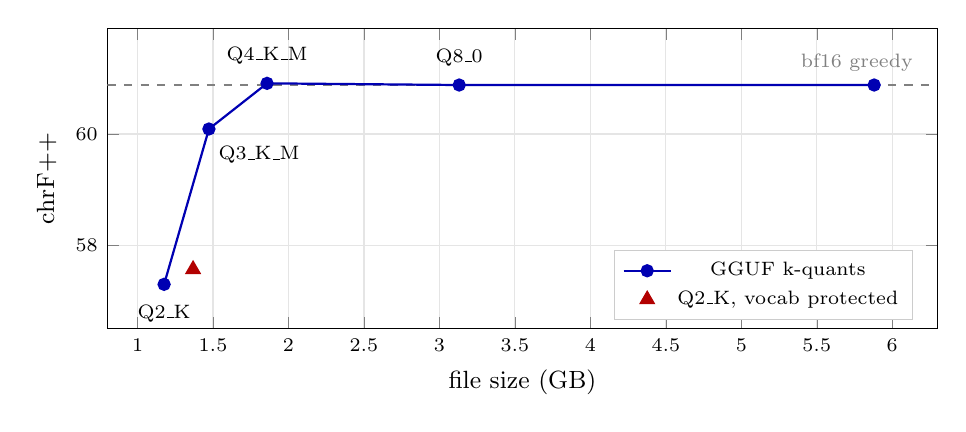
\begin{tikzpicture}
\begin{axis}[
  width=\columnwidth, height=5.4cm,
  xlabel={file size (GB)}, ylabel={chrF++},
  xmin=0.8, xmax=6.3, ymin=56.5, ymax=61.9,
  grid=major, grid style={gray!20},
  legend pos=south east, legend style={font=\scriptsize, draw=gray!40},
  tick label style={font=\scriptsize}, label style={font=\small},
]
\addplot[dashed, gray, thick, forget plot]
  coordinates {(0.8,60.88) (6.3,60.88)};
\node[font=\scriptsize, gray, anchor=south east] at (axis cs:6.2,60.95) {bf16 greedy};
\addplot[mark=*, thick, blue!70!black] coordinates {
  (1.176,57.30) (1.473,60.09) (1.858,60.91) (3.131,60.88) (5.88,60.88)
};
\addlegendentry{GGUF k-quants}
\addplot[only marks, mark=triangle*, mark size=3pt, red!70!black]
  coordinates {(1.368,57.57)};
\addlegendentry{Q2\_K, vocab protected}
\node[font=\scriptsize, anchor=north] at (axis cs:1.176,57.10) {Q2\_K};
\node[font=\scriptsize, anchor=north west] at (axis cs:1.473,59.95) {Q3\_K\_M};
\node[font=\scriptsize, anchor=south] at (axis cs:1.858,61.08) {Q4\_K\_M};
\node[font=\scriptsize, anchor=south] at (axis cs:3.131,61.05) {Q8\_0};
\end{axis}
\end{tikzpicture}
\caption{Quality against file size on the full 1{,}500-pair devtest,
greedy decoding. The chrF++ axis is zoomed to the 56.5--62 range so the
small differences are visible. The curve is flat from 5.88~GB down to
1.86~GB and only then turns. Protecting the vocabulary tensors at 2 bits
(triangle) buys back 0.27 chrF++ for 192~MB; spending a similar amount on
the body instead (Q2\_K to Q3\_K\_M, 298~MB) buys back 2.79.}
\label{fig:curve}
\end{figure}

\subsection{The vocabulary tensors are not the fragile part}
\label{sec:vocab}

Going in, we expected the two $256{,}000 \times 1024$ vocabulary tensors
to be where a Thaana model breaks first. They hold 17.8\% of the
parameters, and they are the layers that map between token identities and
the representation space, so quantizing them coarsely should blur exactly
the distinctions between Thaana tokens. The probes say otherwise, though
not in a symmetric way.

Dropping the token embedding alone from 6 bits to 2, with the rest of the
model kept at Q6\_K, costs only \textbf{0.25} chrF++. Doing the same to
the output projection costs \textbf{0.88}. Both are small next to what
the body costs: moving the body from Q3\_K\_M to Q2\_K gives up 2.79 for
a comparable 298~MB. So the main conclusion is that the vocabulary is not
where this model is fragile. But the two tensors are clearly not
interchangeable either. They have identical shape and size and sit at
opposite ends of the same network, yet one is about 3.5$\times$ more
sensitive than the other.

We think the asymmetry has a simple explanation. The embedding is only
used to look up a vector for each token, and a lookup that lands slightly
off still passes through 32 layers of computation that can absorb the
error. The output projection produces the logits directly: its errors are
the last thing that happens before the argmax picks a token, with nothing
after them to compensate. If that explanation is right, the ordering
should hold for other encoder--decoder models too, and the practical
advice is that llama.cpp's \texttt{--output-tensor-type} option deserves
more care than \texttt{--token-embedding-type}.

Consistent with all this, protecting both vocabulary tensors in an
otherwise 2-bit model (embedding at 8-bit, output projection at 6-bit,
costing 192~MB) recovers only 0.27 of the 3.58 chrF++ lost. Spending
those megabytes on the body instead buys roughly ten times as much. The
rule that falls out is simple: spend bits on the body.

We also want to be honest about something that almost misled us. On the
150-sentence screen, these two probes measured $-0.35$ and $-0.24$, which
put the embedding on the \emph{wrong} side of the comparison and made
both look like noise. The full test set separates them cleanly and
reverses the ordering. Screening was still the right way to spend our
compute, because it correctly picked which artifacts deserved a full run.
But on differences under one chrF++ point, a 150-sentence screen resolved
neither the size nor even the sign of the effect, and we would not have
been comfortable publishing either number from the screen alone.

\section{Speed and memory}
\label{sec:speed}

\begin{table}[t]
\centering\small
\setlength{\tabcolsep}{4pt}
\begin{tabular}{lrrr}
\toprule
Configuration & Peak mem. & \multicolumn{2}{c}{tokens/s} \\
\cmidrule(l){3-4}
              &           & GPU & CPU \\
\midrule
tf.\ bf16, beam 4 & 8.82\,GB$^{\ast}$ & 108 & --- \\
tf.\ bf16, greedy & 6.63\,GB$^{\ast}$ & 148 & --- \\
tf.\ NF4, beam 4  & 6.03\,GB$^{\ast}$ &  76 & --- \\
tf.\ int8, beam 4 & 6.95\,GB$^{\ast}$ &  32 & --- \\
\midrule
GGUF Q8\_0    & 3.93\,GB & 163 & 17.6 \\
GGUF Q6\_K    & 3.28\,GB & 169 & 19.9 \\
GGUF Q4\_K\_M & 2.79\,GB & 178 & 22.7 \\
GGUF Q3\_K\_M & 2.44\,GB & 168 & 24.9 \\
GGUF Q2\_K    & 2.17\,GB & 184 & 29.1 \\
\bottomrule
\end{tabular}
\caption{Throughput and peak memory on a 64-sentence subset. tf.\ =
transformers. $^{\ast}$transformers peak memory is
\texttt{torch.cuda.max\_memory\_allocated}, which excludes the CUDA
context; GGUF peak memory is sampled from \texttt{nvidia-smi} and
includes it, so the GGUF column is if anything pessimistic. transformers
rates are totals over batches of 16; llama.cpp decodes one stream. CPU is
8 threads with no GPU offload.}
\label{tab:speed}
\end{table}

Two patterns in Table~\ref{tab:speed} matter in practice.

\textbf{On a GPU, quantization buys memory, not speed.} Decode rates
across the whole GGUF ladder sit in a narrow band of 163 to 184 tokens/s,
even though the files differ by a factor of 2.7. At this model size the
decode loop is not limited by how fast weights can be read, so smaller
weights do not make it faster. What changes is the footprint: the whole
llama.cpp process peaks at 2.79~GB at Q4\_K\_M, against 8.82~GB for bf16
beam-4 generation in PyTorch.

bitsandbytes helps peak memory much less than its weight compression
suggests. NF4 stores the weights in 3.06~GB, but peak allocation only
falls from 8.82 to 6.03~GB, because the unquantized vocabulary tensors,
the activations and the beam-search state are all still there. int8 was
the slowest configuration we measured at 32 tokens/s, a third of plain
bf16, which is a known cost of LLM.int8()'s mixed-precision scheme. For
this model, int8 loses on every axis: it is larger than NF4, slower than
everything else, and no more accurate.

\textbf{On a CPU, quantization does buy speed.} Here the rates follow
bit-width directly, from 17.6 tokens/s at Q8\_0 to 29.1 at Q2\_K, because
CPU decoding is limited by memory bandwidth in exactly the way GPU
decoding is not. At Q4\_K\_M the model does 22.7 tokens/s on eight CPU
threads, which is roughly one news sentence per second, from a 1.86~GB
file, in under 3~GB of RAM, with no GPU involved. That is the build we
would hand to someone who wants to run this model on an ordinary laptop,
and it is the one we recommend.

\section{Discussion and limitations}

Our results are for one model, one language direction, and one test
domain (news). We would guess that the shape of the curve (flat to 4
bits, a knee below it) is typical for a fine-tuned 3B encoder--decoder,
but we cannot generalize the exact knee position from a single system,
and a model fine-tuned on a narrower task might break earlier.

The two tracks are not measured under identical decoding, because
llama.cpp does not implement beam search for encoder--decoder models. We
handled this by measuring both baselines and comparing like with like,
but it means every GGUF number is a greedy number: a Q4\_K\_M deployment
gives up the 0.98 chrF++ that beam search contributes, on top of the
negligible quantization loss. An encoder--decoder beam search in
llama.cpp is the single change that would most improve the deployed
model.

We did not attempt quantization-aware training, distillation to a smaller
student model, or pruning. All three are plausible routes to something
smaller than 1.86~GB without the 3-bit quality loss, and all three
require training, which post-training quantization deliberately avoids.
Since our setting is calibration-free, we also never used the training
data at quantization time; methods like GPTQ and AWQ that do use
calibration data might push the knee lower, if they gain
encoder--decoder support.

Finally, all measurements come from one Windows machine with one GPU.
The quality numbers do not depend on hardware, but the throughput numbers
in Section~\ref{sec:speed} should be read as a single data point, not a
benchmark.

\section{Conclusion}

A 3B English$\to$Dhivehi translation model that scored 61.8 chrF++ in
bfloat16 can be shipped as a 1.86~GB file that scores the same, runs from
a single binary with no Python, and does not need a GPU. Below 4 bits
quantization costs real quality (0.79 chrF++ at 3 bits, 3.58 at 2 bits),
and it fails by repeating valid Thaana or inserting foreign characters
rather than by breaking the script, which means the script-validity check
that serves this language pair well elsewhere cannot detect it. The
256k-token vocabulary tensors, which we expected to be the sensitive part
of a Thaana model, tolerate 2-bit quantization cheaply, though not
equally: the output projection is about 3.5$\times$ more sensitive than
the token embedding despite being the same size, so
\texttt{--output-tensor-type} deserves more care than
\texttt{--token-embedding-type} when quantizing an encoder--decoder
aggressively. It is the body, not the vocabulary, that sets the floor.
For anyone who wants to run this model, Q4\_K\_M is the setting to use.

\paragraph{Artifacts.}
The merge, conversion, quantization and evaluation scripts are in the
project repository at \url{https://github.com/streetsolider/div-translation},
including the GGUF evaluation harness behind every llama.cpp number in
this paper. The quantized models are released at
\url{https://huggingface.co/str33t/madlad400-3b-mt-en-dv-news-v1-GGUF},
and the bf16 LoRA adapter they derive from remains at
\url{https://huggingface.co/str33t/madlad400-3b-mt-en-dv-news-v1}.

\bibliographystyle{plainnat}
\bibliography{references}

\end{document}
